%
%  $Author: ienne $
%  $Date: 1995/09/15 15:20:59 $
%  $Revision: 1.4 $
%

% \documentclass[10pt,journal,cspaper,compsoc]{IEEEtran}   %%%tc version
\documentclass[10pt, conference]{IEEEtran}
%\documentclass[conference,compsoc]{IEEEtran}
%\documentclass[10pt, conference]{IEEEtran}
%\documentclass[times, 10pt,onecolumn]{article}
\usepackage{amsmath, amssymb, enumerate}

%%%%%%%%%%%%%%%% page control%%%%%%%%%%%%%%%%%
%\usepackage[margin=0.75in]{geometry}

%\linespread{0.991}  %%%%%%%%%%%%%%%%%%%%%%%%%%%%%%%%% this is really useful
%\usepackage{cite}
\usepackage{fancybox}
\usepackage{amsfonts}
%\usepackage{algorithm}
%\usepackage[noend]{algorithmic}
\usepackage[usenames]{color}
%\usepackage{colortbl}
%\usepackage[ figure, boxed, vlined]{algorithm2e}
%\usepackage[linesnumbered,vlined]{algorithm2e}
%\usepackage[lined,boxed]{algorithm2e}
\usepackage{listings}

\usepackage[linesnumbered,vlined]{algorithm2e}
\usepackage{graphicx}
\usepackage{times}
\usepackage{psfrag}
\usepackage{subfigure}
\usepackage{caption}
%\usepackage{subcaption}
\usepackage{multirow}
%\usepackage{setspace}
%\usepackage{listings}
\usepackage{epsfig}
%\usepackage{epstopdf}
%\usepackage[font=small,labelfont=bf]{caption}
\usepackage{url}

\usepackage{color}
\def\fixme#1{\typeout{FIXED in page \thepage : {#1}}
%\bgroup \color{red}{} \egroup}
\bgroup \color{red}{[FIXME: {#1}]} \egroup}


%\usepackage[pdftex]{hyperref}
\usepackage{rotating,tabularx}

\interfootnotelinepenalty=10000

%% Define a new 'leo' style for the package that will use a smaller font.
\makeatletter
\def\url@leostyle{%
  \@ifundefined{selectfont}{\def\UrlFont{\sf}}{\def\UrlFont{\small\ttfamily}}}
\makeatother

%\documentstyle[times,art10,twocolumn,latex8]{article}

%-------------------------------------------------------------------------
% take the % away on next line to produce the final camera-ready version
\pagestyle{plain}
%\thispagestyle{empty}
%\pagestyle{empty}

\newtheorem{theorem}{Theorem}
\newtheorem{lemma}[theorem]{Lemma}

%% remaining budget share, used in task stall section.
\newcommand{\bottomrule}{\hline}
\newcommand{\toprule}{\hline}
\newcommand{\midrule}{\hline}
%-------------------------------------------------------------------------
\begin{document}

\title{DeepPicar:​ ​A​ ​Low-cost​ ​Deep​ ​Neural​ ​Network-based​ ​Autonomous​ ​Car}
\author{Author One, Author Two\\
\{author1,author2\}@ku.edu\\
University of Kansas, USA\\ 
}

\maketitle
\thispagestyle{empty}
\begin{abstract}

Abstract goes here.

\end{abstract}

%-------------------------------------------------------------------------

\section{Introduction} \label{sec:intro}

% broad context:
% - advance in ai sparked interests in the robotics application, such as
%   self-driving cars.
% - in particular, deep neural network models are increasingly used
%   for perception and control of a vehicle. say. AI workloads.
%
%
Autonomous cars have been a topic of increasing interest in recent
years as many companies are actively developing related hardware
and software technologies toward fully autonomous driving capability without
any human intervention. Deep neural networks (DNNs) have been
sucessfully applied in various perception and control tasks in 
recent years, and they are important workloads for autonomous vehicles
as well. For example, Tesla Model S was known to use a specialized
chip (MobileEye EyeQ), which uses a deep neural network for vision-based
real-time obstacle detection and avoidance. More recently, researchers
are investigating DNN based end-to-end control of
cars~\cite{Bojarski2016} and other robots. It is expected that more
DNN based Artifical Intelligence workloads may be used in future
autonomous vehicles.

% big problem
Executing these AI workloads on a embedded computing platform that can
be used in a car poses several additional challenges. First, many AI
workloads in vehicles are computationaly demanding and have strict
real-time requirements. For example, latency in a vision-based object
detection task may directly linked to safety of the vehicle. This
requires a high computing capacity as well as means to guaranteeing
the timings. On the other hand, the computing hardware platform must
also satisfy cost, size, weight, and power constraints, which require
highly efficient computing platform. These two conflicting
requirements  complicate the platform selection process as observed in
~\cite{Otterness2017}, which evaluated vision workloads on
NVIDIA's Tegra TX1 platform.
%% For example, while today's self-driving car
%% prototype equip more \$100,000 
%% of computers and sensors~\cite{juliussen2014emerging}, a study
%% found that aveage consumers are willing to pay much less amount of
%% extra cost for a self-driving capability~\cite{Daziano2017}.
%% https://qz.com/924212/what-it-really-costs-to-turn-a-car-into-a-self-driving-vehicle/ 

% related work and remaing problems
To understand what kind of computing hardware is needed for AI
workloads, we need a testbed and realistic workloads. While a real car
testbed would be most ideal, it is not only highly expensive but also
poses serious safety concerns that hinder development and exploration.
Therefore, there is a strong need for safer and less costly testbeds
that still employ state-of-the-art AI technologies. There are already
several relatively inexpensive RC-car based testbeds, such as MIT
RaceCar~\cite{shin2017project} and UPenn's F1$/$10 racecar~\cite{upennf1tenth}.
However, these RC-car testbeds still cost more than \$3,000.

% our goals
Instead, we want to build a low cost testbed that still employs the
state-of-the art AI technologies. Specifically, we focus on a deep
convolutional neural network (CNN) based end-to-end control system,
which was developed for a real self-driving car, NVIDIA
DAVE-2~\cite{Bojarski2016}, and use the same moethodology on a
smaller, safer and less costly setup. In developing the testbed, our
goals are (1) to analyze real-time issues in DNN based end-to-end
control; (2) to evalute real-time performance of contemporarly embedded
multicore platforms for the AI workloads.

% DeepPicar introduction
In this paper, we present DeepPicar, a low-cost autonomous car
platform for research and education. From hardware perspective, 
DeepPicar is comprised of a Raspberry Pi 3 Model B quad-core
computer, a web camera and a RC car, all of which are affordable
components (less than \$100 in total).
The DeepPicar, however, employs state-of-the-art AI
techonologies, including a vision-based end-to-end control system that
utilizes a deep convolutional nueral network (CNN).
The network receives an image frame from a single forward
looking camera as input and generates a predicted steering angle
value as output at each control period in \emph{real-time}. 
The network has 9 layers, about 27 million connections
and 250 thousand parameters (weights).
The network architecture is identifical to that of NVIDIA's DAVE-2
self-driving car~\cite{Bojarski2016}, which uses much more powerful
computer (Drive PX computer~\cite{drivepx}) than Raspberry Pi~3.
We chose to use Pi 3 not only because of its
affordability but also because it is representative
of today's mainstream low-end embedded multicore platforms, found in
smartphones and other embedded devices.

%% Other than the difference in scale (RC car vs. real car), the only other
%% differences between the two systems---from the computing
%% perspective---are that our system is implemented in
%% TensorFlow~\cite{abadi2016tensorflow} and runs on a Raspberry Pi 3
%% whereas NVIDIA's DAVE-2 systems is implemented in Torch
%% 7~\cite{collobert2011torch7} and runs on a Drive PX computer (NVIDIA's
%% automotive specialized computing system~\cite{drivepx}), which is more
%% powerful but also more expensive.

% how we trained (maybe moved to a later section)
We apply a standard imitation learning methodology to train the cat to
follow tracks on the ground. We collect data for 
taining and validation by manually  
controlling the RC car and recording the vision (from the webcam
mounted on the RC-car) and the human control inputs. We then train the
network offline using the collected data on a desktop computer, which
equips a NVIDIA GTX 1060 GPU. Finally, the trained network is copied
back to the Raspberry Pi, which is then used to perform interference
operations---locally on the Pi---in the car's main control loop in
real-time. For real-time control, each inference operation must
be completed within the desired control period. (e.g., 50ms period for
20Hz control frequency.)
% how we evaluated (in terms real-time performance)

% what are our findings?
\fixme{TBD: Summary of our findings}

% contributions
The {\bf contributions} of this paper are as follows:
\begin{itemize}
  \item We present the design and implementation of a
    low-cost autonomous vehicle testbed DeepPicar, which utilizes the
    state-of-the-art aritificial intelligence techniques.
  \item We provide an analysis and case-study of real-time issues in the
    DeepPicar.
  \item We systematically compare real-time computing capabilities of
    multiple embedded computing platforms in the contex of a
    vision-based autnomous driving.
\end{itemize}

%% The DeepPicar is comprised of a Raspberry
%% Pi 3 Model B, a camera and a low cost RC car.

%% By creating and using the Picar platform, we seek to accomplish the 
%% following three goals. First, the significant reduction of the overall
%% cost required 
%% would make autonomous driving research more accessible to interested
%% individuals/parties. Furthermore, it would remove the concerns of
%% creating replacement platforms as each part, or the entire system,
%% could be replaced relatively inexpensively. Second, the utilization of
%% a more cost-efficient platform would allow for a better understanding
%% of the performance requirements necessary for efficiently operating
%% autonomous vehicles. Finally, we strive to achieve the ability to
%% compare the real-time performance of multiple embedded computing
%% platforms. 

%% We display the efficacy of the Picar by training and testing the
%% DeepTesla DNN \cite{} in a custom-made environment. We find that the
%% Picar is capable of consistently accomplishing all real-time
%% operations required for autonomous driving in a 50 millisecond frame. 

The remaining sections of the paper are as follows: Section II gives
an overview of the platform, including the high-level system and the
methods used for training and inference. Section III discusses the
ways/methodologies in which training data was collected. Section IV
outlines the network architecture. This is followed by the real-time
DNN inferencing in Section V. Section VI reviews the online/offline
training done with the platform, with an evaluation given in Section
VII. Section VIII gives a discussion of related works, and the paper
finishes with conclusions in Section IX. 


%% it is necessary that all real-time operations are successfully
%% performed prior to their deadlines. This requires that the AV platform
%% be capable of completing all necessary computations in a timely
%% manner, while maintaining a high level of accuracy. Consequently, the
%% cost of creating a platform capable of self-driving can be relatively
%% high, especially in the current cost-sensitive climate of the
%% automotive industry \cite{}. The overall price for an autonomous
%% vehicle platform currently acts as a bottleneck, especially from an
%% academic standpoint, where cost is an important factor. For many
%% researchers and students, the charge associated with autonomous
%% vehicle research is a significant barrier. These same parties may also
%% be deterred from participating in autonomous vehicle research due to
%% the potential for their developed platforms to break in the
%% experimental process. The idea of building one relatively expensive
%% platform may not be too daunting for some, but the notion of
%% potentially making multiple identical platforms in case of accidents
%% may be overwhelming.
%% Toward this end, we explore the possibility of
%% developing a low-cost system that still employs state-of-the-art AI
%% technologies and is capable of executing real-time autonomous vehicle
%% operations. 


\section{Background and Related Work} \label{sec:background}

In this section, we provide background and related work on the
application of deep learning in robotics, particularly autonomous
vehicles. 

\subsection{End-to-End Deep Learning for Autonomous Vehicles}

%% - explosion of AI
%% - in particular, application of DNN in perception and control of robotics systems.
%% - end-to-end control is a promising technique.
%%   levine's publications?
%% - examples: nvidia's DAVE-II prototype, forest navigating drone
%% challenge problem: computing at low cost?

To solve the problem of autonomous driving, a standard approach has
been decomposing the problem into multiple sub-problems,
such as lane marking detection, path planning, and low-level
control, which together form a processing pipeline~\cite{Bojarski2016}.
Recently, researchers are exploring another approach that dramatically
simplifies the standard control pipeline by applying deep neural
networks to directly produce control outputs from senor
inputs~\cite{Levine2016}. Figure~\ref{fig:end-to-end-control}
shows the differences between the two approaches.

\begin{figure}[h]
  \centering
  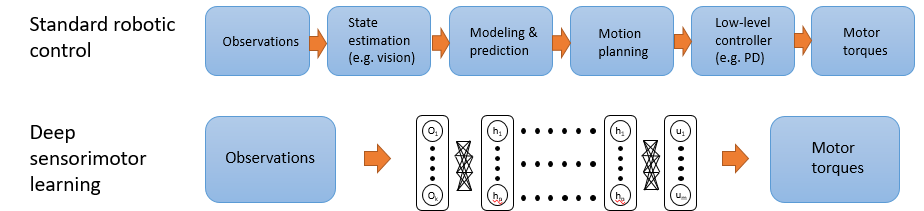
\includegraphics[width=.75\textwidth]{figs/endtoend_redrawn}
  \caption{Standard robotics control vs. DNN based end-to-end
    control. Adopted from ~\cite{Levine2017cs294}.}
  \label{fig:end-to-end-control}
\end{figure}

The use of neural networks for end-to-end control of autonomous
car was first demonstrated in late 1980s~\cite{Pomerleau1989},
using a small 3-layer fully connected neural network; and subsequently
in a DARPA Autonomous Vehicle (DAVE) project in early
2000s~\cite{LeCun:04}, using a 6 layer convolutional neural network
(CNN); and most recently in NVIDIA's DAVE-2
project~\cite{Bojarski2016}, using a 9 layer CNN. In all of these projects,
the neural network models take raw image pixels as input and directly
produce steering control commands, bypassing all intermediary steps and
hand-written rules used in the conventional robotics control approach.  
NVIDIA's latest effort reports that their trained CNN
autonomously controls their modified cars on public roads without human
intervention~\cite{Bojarski2016}.

Using deep neural networks involves two distinct
phases~\cite{NVIDIA2015}. The first
phase is \emph{training} during which the weights of the network are
incrementally updated by backpropagating errors it sees from the
training examples. Once the network is trained---i.e., the weights of
the network minimize errors in the training examples---the next phase
is \emph{inferencing}, during which unseen data is fed to the network
as input to produce predicted output (e.g., predicted image
classification). In general, the training phase is more computationally
intensive and requires high throughput, which is generally not
available on embedded platforms. The inferencing phase, on the
other hand, is relatively less computationally intensive and latency becomes
as important, if not moreso, as computational throughput, because many
use-cases have strict real-time requirements (e.g., search query
latency).

%% \cite{Levine2016}: ``In this paper, we aim to answer
%% the following question: does training the perception and control
%% systems jointly end-toend 
%% provide better performance than training each component separately?''

%% \cite{Bojarski2016} nvidia paper
%% ``We trained a convolutional neural network (CNN) to map raw pixels from
%% a sin- gle front-facing camera directly to steering commands.''

%% ``Compared to explicit decomposition of the problem, such as lane
%% marking detec- tion, path planning, and control, our end-to-end system
%% optimizes all processing steps simultaneously. We''

%% UPenn's f1/10 BOM: $3,628.37
%% http://f1tenth.org/
%% http://selfdrivingcars.mit.edu/
%% http://fast.scripts.mit.edu/racecar/
%% https://github.com/mit-racecar
%% https://mit-racecar.github.io/

\subsection{Embedded Computing Platforms for Real-Time Inferencing}
Real-time embedded systems, such as an autonomous vehicle, present
unique challenges for deep learning, as the computing platforms of such
systems must satisfy two often conflicting goals~\cite{Otterness2017}:
%% Recent successes in AI, including NVIDIA's DAVE-2 showing, are due
%% in large part to the increased computing performance,
%% which afforded researchers to train and use ever deeper neural networks with
%% high accuracy.
%% For practical applications, the computer platform in an
%% autonomous vehicle must satisfy two often conflicting goals:
The platform must provide 
enough computing capacity for real-time processing of computationally
expensive AI workloads (deep neural networks);
The platform must also satisfy various
constraints such as cost, size, weight, and power consumption limits.

Accelerating AI workloads, especially inferencing
operations, has received a lot of attention from academia and industry
in recent years as applications of deep learning are broadening to
areas of real-time embedded systems such as autonomous vehicles. These
efforts include the development of various heterogeneous architecture-based 
system-on-a-chips (SOCs) that may include multiple cores, GPU,
DSP, FPGA, and neural network optimized ASIC hardware~\cite{Jouppi2017}.
Consolidating multiple tasks on SoCs with lots of shared hardware
resources while guaranteeing real-time performance is also an active
research area, which is orthogonal to improving raw
performance. Consolidation is necessary for efficiency, but unmanaged 
interference can nullify the benefits of consolidation~\cite{Kim2016}.
For these reasons, finding a good computing platform is a
non-trivial task, one that requires a deep understanding of the
workloads and the hardware platform being utilized.

The primary objectives of this study are to understand (1) the
necessary computing performance for applying AI technology-based
robotics systems, and (2) what kind of computing architecture and
runtime supports are most appropriate for such workload. To
achieve these goals, we implement a low-cost autonomous car platform
as a case-study and systematically conduct experiments, which we will 
describe in the subsequent sections.


\section{DeepPicar Overview}\label{sec:overview}

In this section, we provide an overview of our DeepPicar platform.
In developing DeepPicar, one of our primary goals is to faithfully
replicate NVIDIA's DAVE-2 system on a smaller scale using a low cost
multicore platform, the Raspberry Pi 3. Because Raspberry Pi 3's
computing performance is much lower than that of the DRIVE
PX~\cite{drivepx} platform used in DAVE-2, we are interested in if,
and how, we can process 
computationally expensive neural network operations in
real-time. Specifically, inferencing (forward pass processing)
operations must be completed within each control period
duration---e.g., a WCET of 33.3 ms for 30Hz control 
frequency---locally on the Pi 3 platform, although training of the 
network (back-propagation for weight updates) can be done offline and 
remotely using a desktop computer.

\begin{figure}[h]
  \centering
  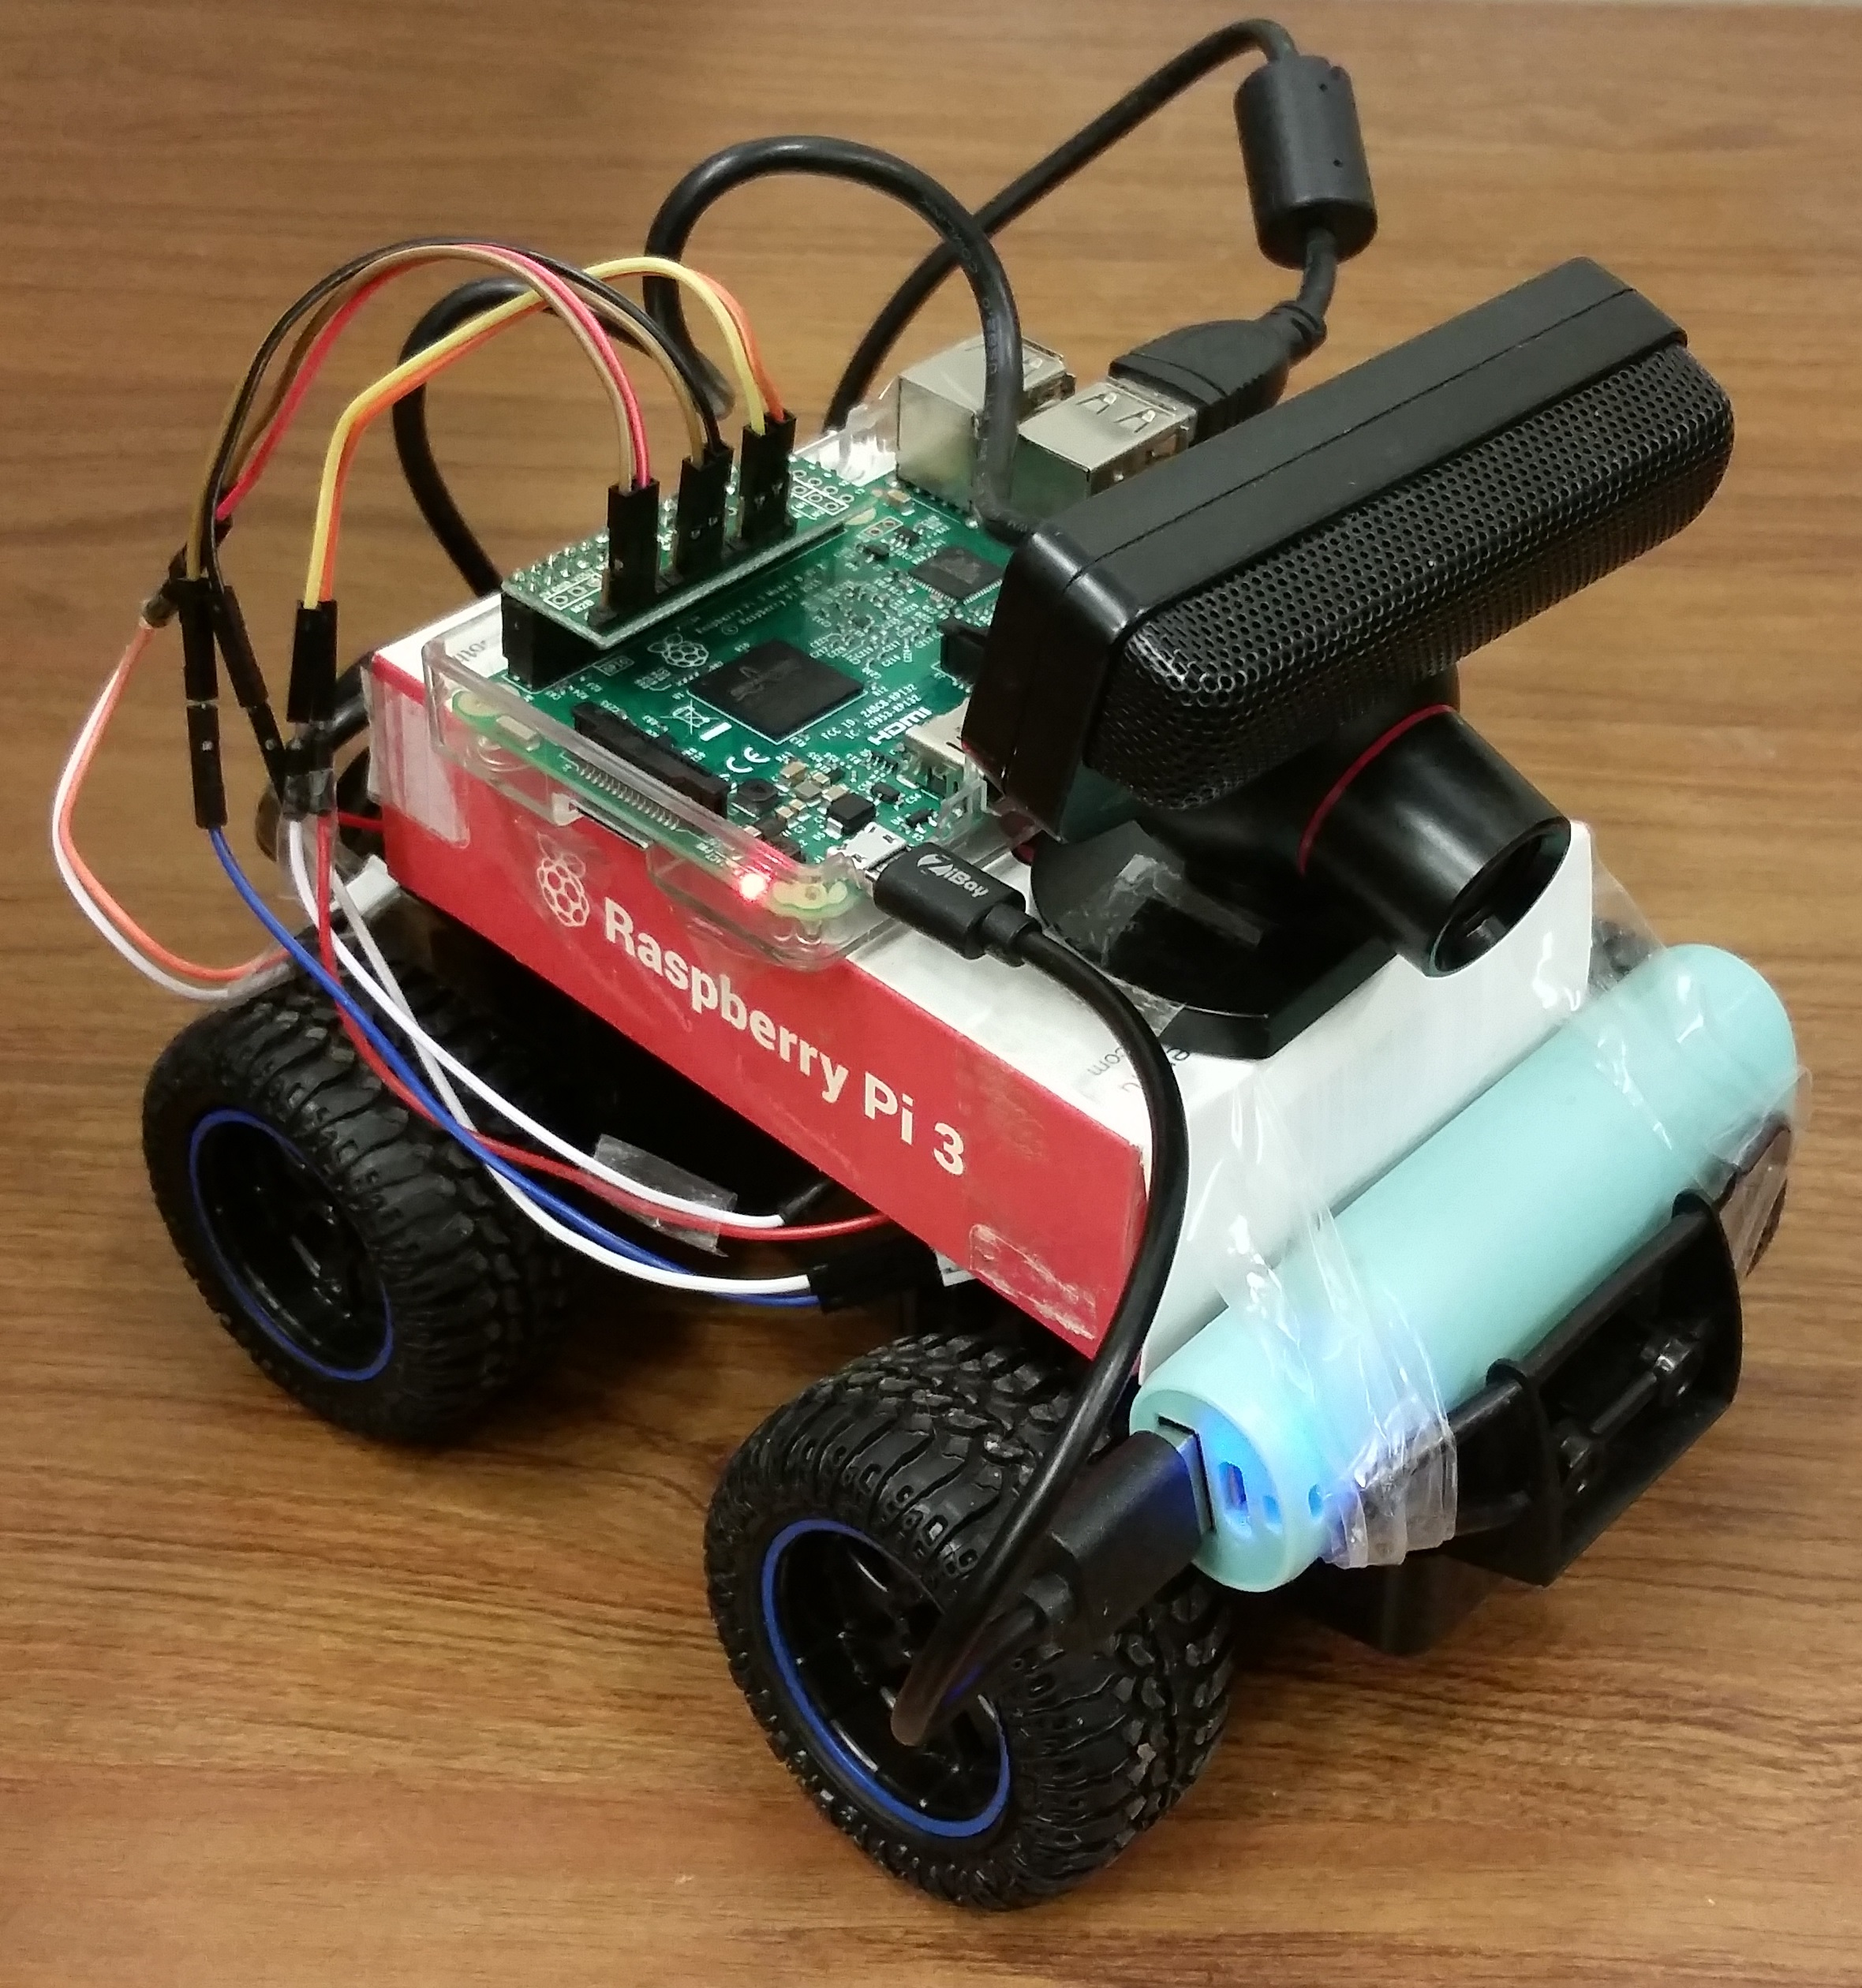
\includegraphics[width=.4\textwidth]{figs/DeepPicar_platform}
  \caption{DeepPicar platform.}
  \label{fig:overview}
\end{figure}

\begin{table}[h]
  \centering
  \begin{tabular}{|c|r|}
    \hline
    Item                    & Cost (\$) \\
    \hline
    Raspberry Pi 3 Model B  & 35 \\
    New Bright 1:24 scale RC car       & 10 \\
    Playstation Eye camera  &  7 \\
    Pololu DRV8835 motor hat&  8 \\
    External battery pack \& misc.   & 10 \\
    \hline
    Total                   & 70 \\
    \hline
  \end{tabular}
  \caption{DeepPicar's bill of materials (BOM)}
  \label{tbl:carbom}
\end{table}

Figure~\ref{fig:overview} shows the DeepPicar, which is comprised of a
set of inexpensive components: a Raspberry Pi 3 Single Board Computer
(SBC), a Pololu DRV8835 motor driver, a Playstation Eye webcam, a
battery, and a 1:24 scale RC car. Table~\ref{tbl:carbom} shows the
estimated cost of the system.

For the neural network architecture, we implement NVIDIA DAVE-2's
convolutional neural network (CNN) using an open-source CNN model in
~\cite{deeptesla}. Note, however, that the CNN model
in~\cite{deeptesla} is considerably larger than NVIDIA's CNN
model as it contains an additional fully-connected layer of
approximately 1.3M additional parameters. We remove the additional
layer to faithfully recreate NVIDIA's original CNN model.
%% The main difference is that we do not utilize a normalization layer, and 
%% instead initialize the weights using a Xavier initialization. 
As in DAVE-2, the CNN takes a raw color image (200x66 RGB pixels)
as input and produces a single steering angle value as output.
Figure~\ref{fig:architecture} shows the network architecture
used in this paper, which is comprised of 9 layers, 250K parameters,
and about 27 million connections as in NVIDIA DAVE-2's architecture.

\begin{figure}[h]
  \centering
  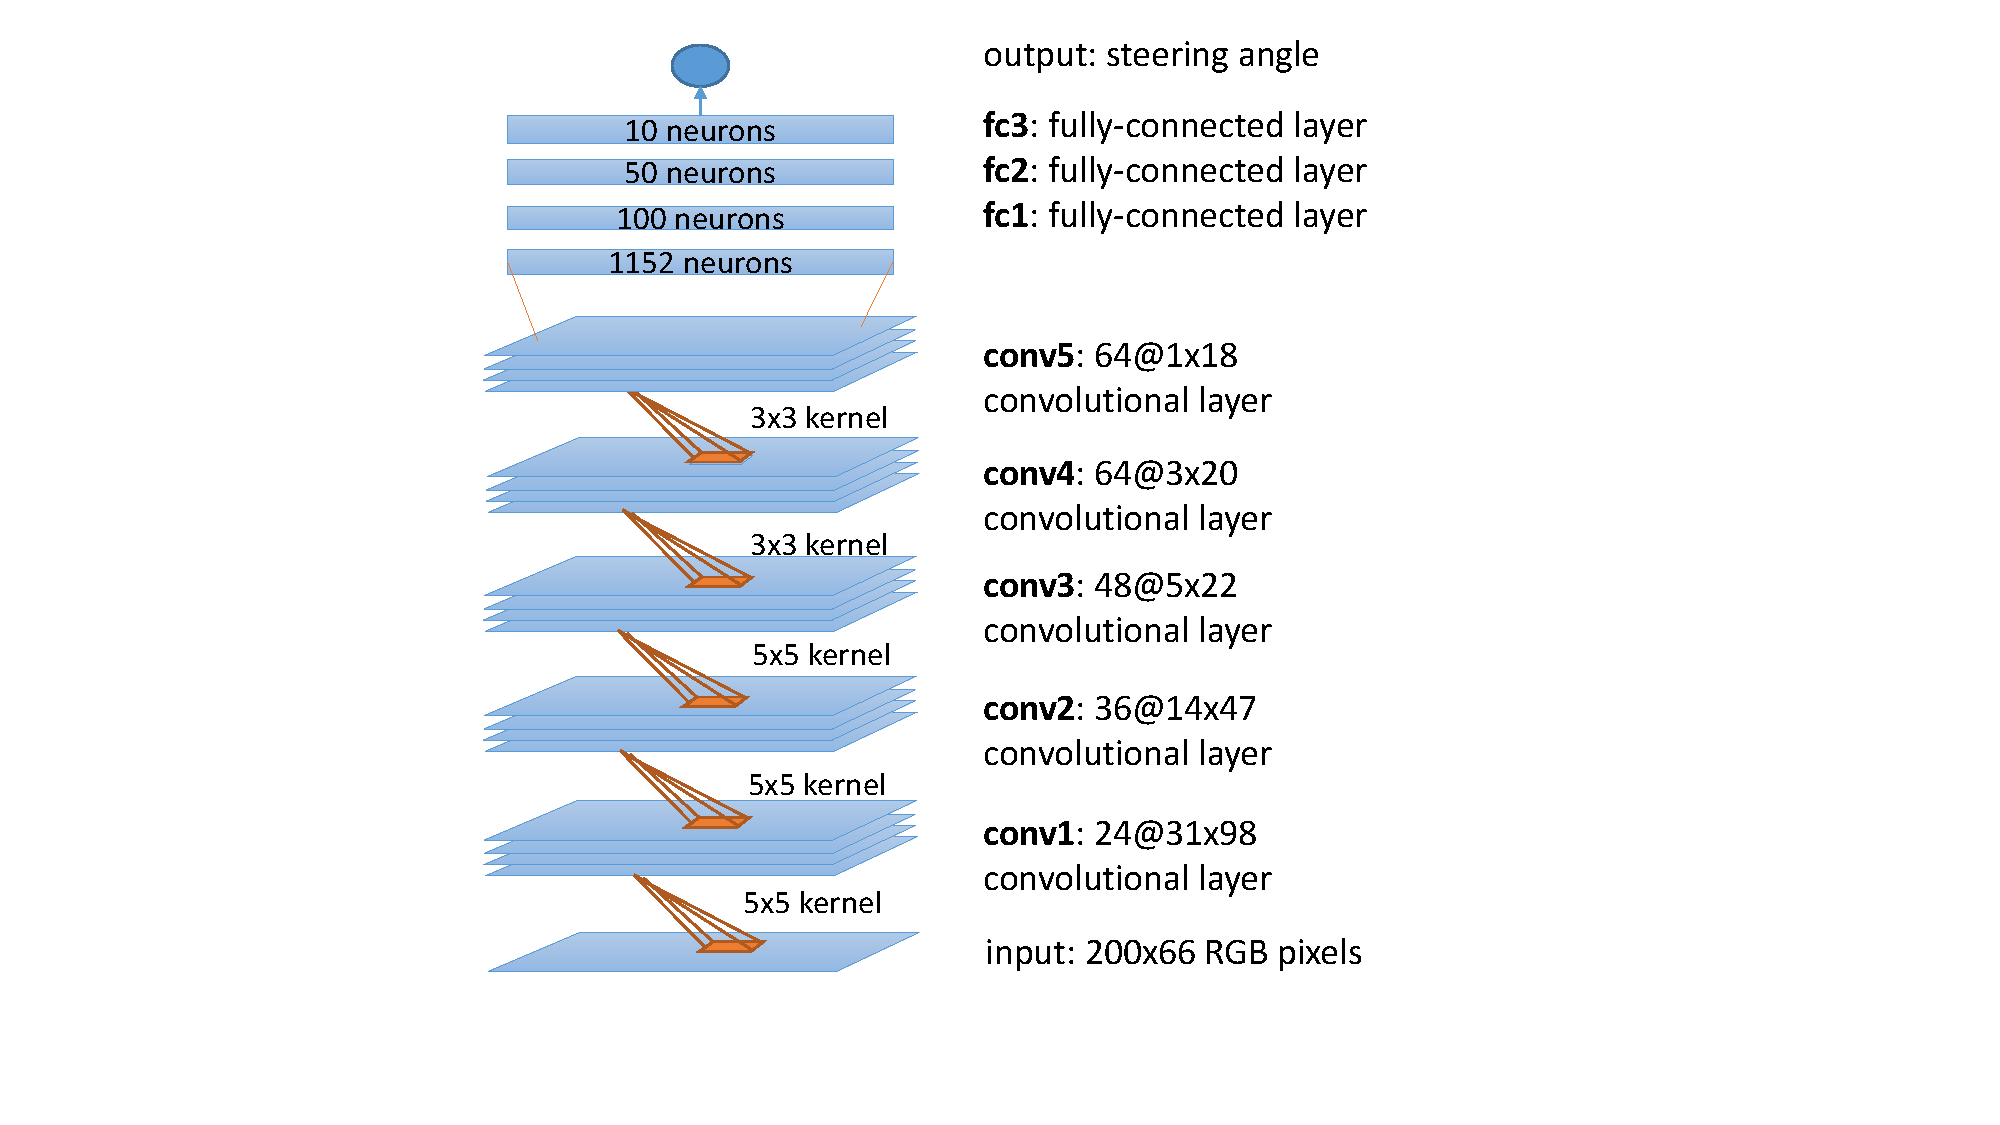
\includegraphics[width=0.4\textwidth]{figs/architecture}
  \caption{DeepPicar's neural network architecture: 9 layers (5
    convolutional, 4 fully-connected layers), 27 million connections,
    250K parameters. The CNN architecture is identical to the one 
	used in NVIDIA's real self-driving car~\cite{Bojarski2016}.}
  \label{fig:architecture}
\end{figure}


%% Note, however,
%% that we did not apply the normalization mentioned
%% in~\cite{Bojarski2016}, as it does not include trainable parameters
%% and its computational demand with respect to the overall CNN
%% processing is minimal.

\begin{figure}[h]
  \centering
  \begin{subfigure}{0.4\textwidth}
    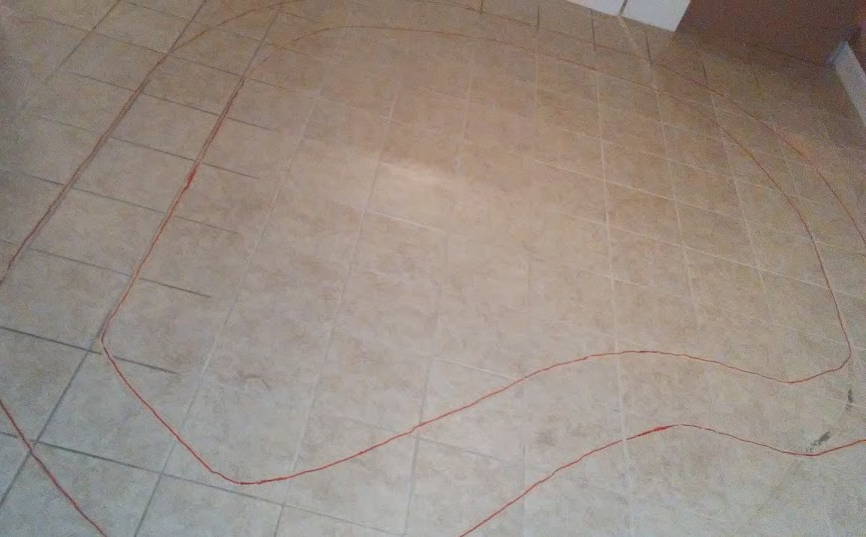
\includegraphics[width=\textwidth]{figs/track-2}
    \caption{Track 1.}
    \label{fig:track}
  \end{subfigure}
  \hfill
  \begin{subfigure}{0.4\textwidth}
    \includegraphics[width=\textwidth]{figs/track-3}
    \caption{Track 2.}
    \label{fig:track2}
  \end{subfigure}
  \caption{Custom tracks used for training/testing}
  \label{fig:tracks}
\end{figure}

% data collection and training.
To collect the training data, a human pilot manually drives the RC car
on tracks we created (Figure~\ref{fig:tracks}) to record
timestamped videos and contol commands. The stored data is then copied 
to a desktop computer, which is equipped with a NVIDIA Titan Xp GPU, 
where we train the network to accelerate training speed.

%% For comparison, training the network on the Raspbeery Pi 3 takes
%% approximately 4 hours, whereas it takes only about 4 minutes on the
%% desktop computer using the Titan Xp GPU.

\begin{figure}[h]
   \lstset{language=python,
           basicstyle=\ttfamily\small,
           keywordstyle=\color{blue}\ttfamily,
           stringstyle=\color{red}\ttfamily,
           commentstyle=\color{green}\ttfamily
          }  
  \lstinputlisting[language=python]{control.py}
  \caption{Control loop}
  \label{fig:controlloop}
\end{figure}

% inferencing on pi3
Once the network is trained on the desktop computer, the trained model
is copied back to the Raspberry Pi 3. The network is then used
by the car's main controlller, which feeds image frames from the web
camera as input to the network in real-time. At each control period,
the network produced steering angle output is converted into the PWM values
of the car's steering motor. Figure~\ref{fig:controlloop} shows simplified 
pseudo code of the controller's main loop. Among the five steps, the 3rd step, 
network inferencing, is the most computationally intensive and dominates the
execution time.

Note that although the steering angle output of the network ($angle$) is
a continuous real value, the RC car platform we used only supports
three discrete angles---left (-30$^{\circ}$), center 
(0$^{\circ}$), and right (+30$^{\circ}$)---as control inputs.
We approximate the network generated real-valued angle to the closest
one of the three angles. Although this may introduce inaccuracy in
control, the observed control performance of the system is respectable,
likely due to the inherently stocastic nature of DNN.

%% In the future, we plan to use a different (more expensive) RC car
%% platform that can precisely control the car's steering angle.

Another factors that can potentially affect the prediction accuracy of
the CNN, are camera and actuator (motor) control latencies. The camera
latency is from the time the camera sensor observes the scene to the
time the computer actually reads the digitized image data. This time
can be noticable depending on the camera used and the data processing
time of the computing platform. Higher camera latency could
negatively affect control performance, because the DNN would analyze
stale scenes. The actuator (motor) control latency from the time
the control output is sent to the steering motor to the time the motor
actually moved at a desired position, which also can takes
considerable time. In our platform, the combined latency is measured
to be around 50 ms, which is reasonble.
%% In other words, %% in the recorded video and control data, 
%% a control action of the CNN appears to be applied 50 ms later.
%% Considering that camera's framerate is 30Hz
%% (33.3 ms/frame), this is about two frames after the control action.
%% We experimentally measured the camera
%% latency and found it to be around 50-100 ms.
If this value is too high, control performance may suffer.
Our initial prototype suffered this problem as the observed latency
was as high as 300 ms, which negatively affected control performance.
For reference, the latency of human perception is known to be as fast
as 13 ms~\cite{ThomasBurger2015}. 
% https://www.pubnub.com/blog/2015-02-09-how-fast-is-realtime-human-perception-and-technology/

Our trained DNN models showed good prediction accuracy, successfully
navigating several different tracks we used for training.
For instance, the DeepPicar could remain on Track 1
(Figure \label{fig:track}) over 10 minutes at a moderate speed (50\%
throttle), at which point we stopped the experiment, and more than one
minute at a higher speed (75\% throttle)~\footnote{Self-driving videos: \url{https://photos.app.goo.gl/q40QFieD5iI9yXU42}
  %% \url{https://photos.app.goo.gl/ce93sU7jPk4ywO8u2}
}. Running at
higher speed is inherently more challenging because the CNN controller
has less time to recover from mistakes (bad predictions).  Also, we
find that the prediction accuracy is significantly affected by the
quality of training data as well as various environmental factors such
as lighting conditions. We plan to investigate more systematic ways
to improve the CNN's prediction accuracies.

We would like to stress, however, that
%% the issues related to the
%% CNN's accuracies have no impact on the \emph{computational 
%% aspects of the system}, and that 
our main focus of this study is not in improving the network accuracy
but in closely replicating the DAVE-2's network architecture and
studying its real-time characteristics, which will be presented in the
subsequent section.


\section{Platform Overview}

\begin{figure}[h]
  \centering
  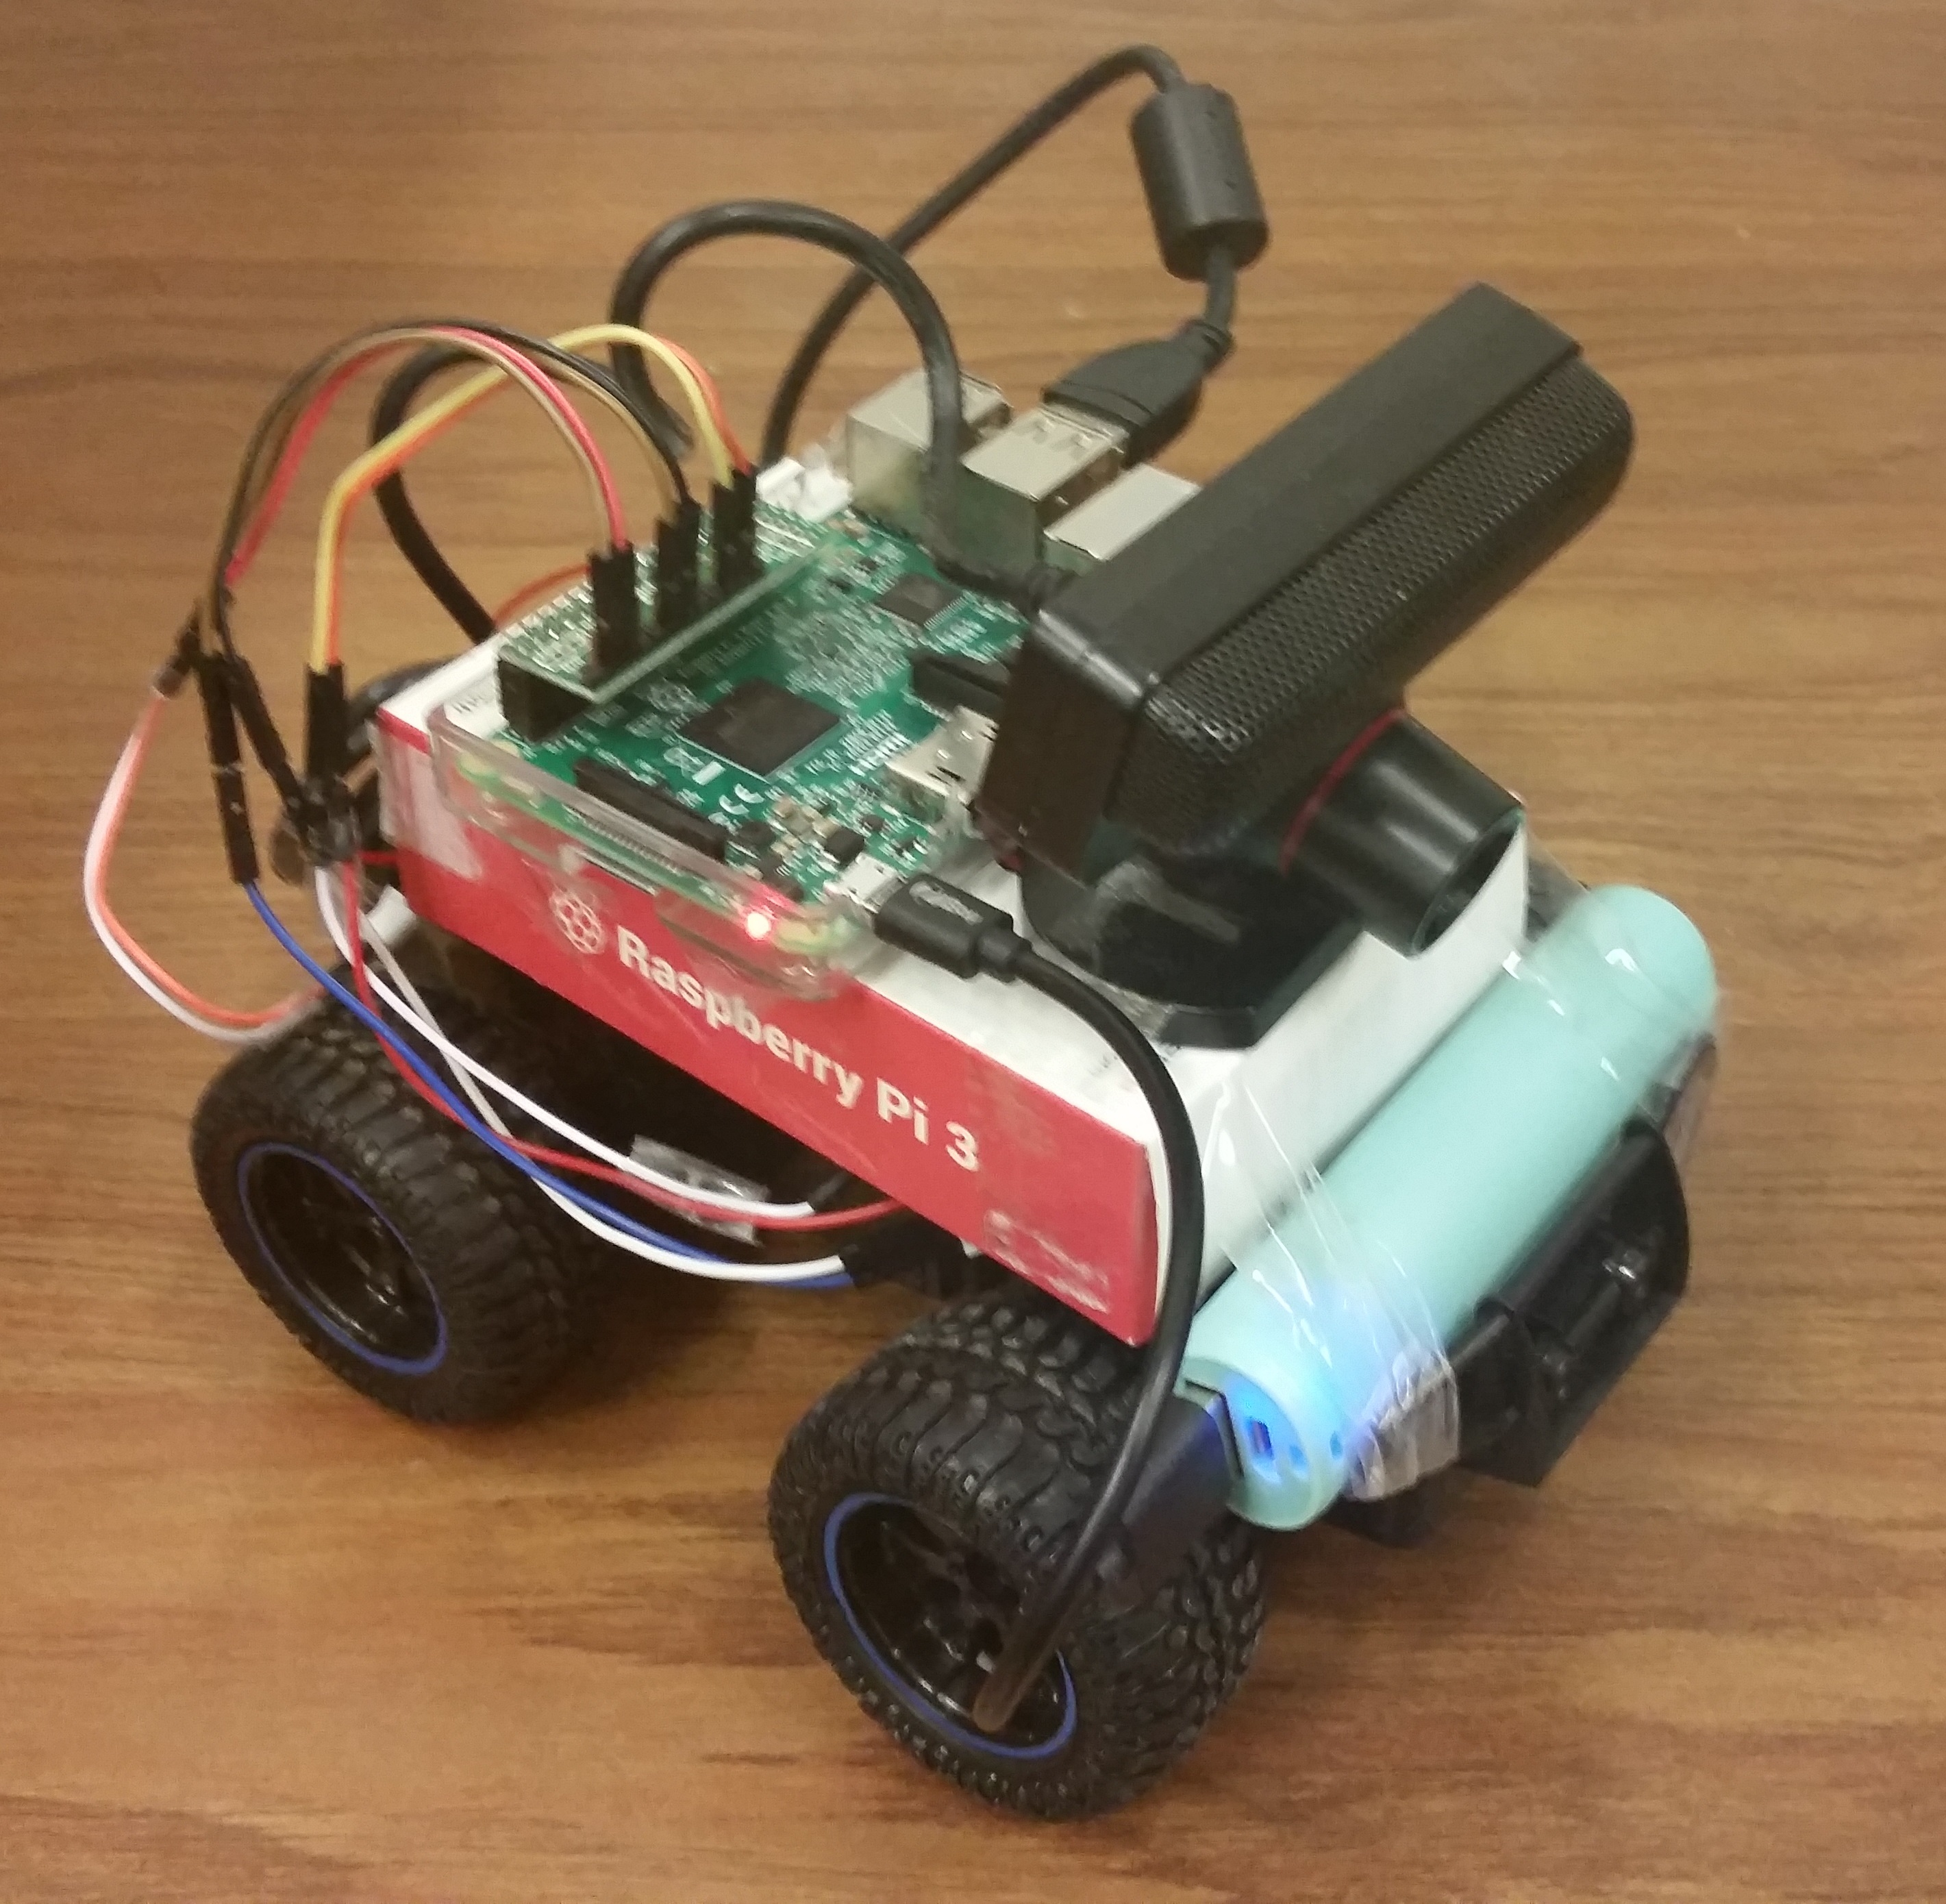
\includegraphics[width=.4\textwidth]{Picar_Picture}
  \caption{ The Picar Platform. }
\end{figure}

\subsection{Platform Components}

\begin{table*}[h]
  \centering
  \begin{tabular} {| l | l | l | l | l |}
    \hline
    \textbf{Platform} & \textbf{Picar} & \textbf{F1/10} & \textbf{NVIDIA DAVE-2}\\ \hline 
    Car & Mini RC Car (\$10) & Traxxas 1/10th car platform (\$299.97) & TBD\\ \hline
    Embedded system & Raspberry Pi 3 Model B (\$35.00) & NVIDIA Jetson TK1 (\$192.99) & NVIDIA DRIVE PX \\ \hline
    CPU & Cortex A-53 quad core & Cortex A-15 quad core & 8x Cortex A-57 quad core, 8x Cortex A-53 quad core \\ \hline
    Camera & Playstation Eye camera (\$6.99) & ZED camera (\$449.00) & 3x cameras\\ \hline
    Power Supply & Mobile battery (\$5.99) & Energizer battery pack (\$159.00) & TBD\\
    \hline
  \end{tabular}
  \caption{Comparison of components used in autonomous vehicle platforms.}
\end{table*}

We employ a small and relatively inexpensive RC car that is capable of performing basic automotive 
operations. However, the car we use doesn't replicate the capabilities of other autonomous vehicle 
platforms, as it is more simplistic in nature. Notably, the RC car we use only has three possible 
options in terms of turning: center, left, and right. As such, control of the car may be less precise at 
times, and may negatively affect performance. The car is capable of other operations that aren't used 
within the scope of this platform. Specifically, the car is able to drive in reverse and the driving 
speed can be changed. In our experiments, we have the RC car drive forward, and at a constant speed.

Our platform also comes equipped with a camera that is used for both recording training videos and 
providing input frames to the model whenever the Picar is self-driving. We chose the Playstation Eye 
Camera due to its ability to reach and maintain higher fps levels while also remaining relatively 
low-cost. One concern, however, is the affect of camera latency on the self-driving performance of our 
platform. While humans are able to see environmental changes in real-time, the same can't be said for 
cameras since there is a delay between when frame capture by the camera, and when it is read by the 
Raspberry Pi 3. As a result, it is possible for the model to be given an input frame that is different 
from the real world, thus impacting the performance of the Picar.

Compared to other existing autonomous vehicle platforms, such as the F1/10 and NVIDIA DAVE-2, the Picar 
platform is capable of performing the same operations while using more cost inexpensive components. As 
shown by Table 1, the components selected for the Picar all cost considerably less than the other 
platforms when focusing on the common components (camera, power supply, etc.). Including the other 
components used in the F1/10 and DAVE-2, such as the additional sensors employed by both, the difference 
in cost would be even greater.

\subsection{Model Training}
In order to operate the Picar as an autonomous vehicle, we utilize the DeepTesla library, which is 
capable of training a deep neural network (DNN) with end-to-end learning, that could then be used by the 
Picar for autonomous driving. Please note that it is more efficient to execute the actual model training 
process on a different system with an NVIDIA GPU, rather than on the Raspberry Pi 3 itself. This is 
because DeepTesla trains the DNN with the Tensorflow library, which greatly benefits from the use of 
gpu-enabled operations. For comparison, training a model on the Pi took approximately 6 hours, whereas 
the time it took on a computer with a NVIDIA GPU was only around 5 minutes! 

We train our model on a custom made track/lane composed of black and white duct tape, where the black 
tape represents the bounds of the track, and the white tape marks the center of the lane. The model is 
taught to stay close to the center of the lane for as long as possible, and to turn whenever it 
reaches/crosses the outer lane bounds so that it remains on the track. For data, we navigate and record 
the car going both ways across the track, and use the collected videos to train the model(s) that will 
be used later for angle prediction while the car is self-driving.

\section{Data Collection}
...
\section{Network Architecture}
...
\section{Real-Time DNN Inferencing}
...
\section{Online/Offline Training}
...
\section{Evaluation}
In evaluating the real-time efficacy of the Raspberry Pi 3, the same methodology is utilized in all 
experiments conducted. The performance of the Pi is measured over a set of 1001 video frames that are 
each individually fed to the model. The processing time for the first frame is ignored as, due to 
cache warmup, it is uncharacteristically high and doesn't accurately represent the Pi's capabilities. A 
deadline of 50 ms, or 20 Hz, is used as a baseline to assess the Pi's ability to complete all 
necessary real-time operations in a timely manner. Also, please note that frame processing times 
would be approximately the same if the input stream was a 
camera instead of a video. 

\subsection{Real-Time Operations}
In a real-time operations, the system has to be capable of consistently executing all necessary 
functions before their given deadlines. In the case of our platform, it has to process every given frame 
and get the predicted angles from the model. In order to determine if the Raspberry Pi 3 is capable of 
this, we tested the platform and recorded the time it took for the Pi to complete all real-time 
functions for every given frame.For this experiment, all four of the Pi's cpu cores were utilized, and 
only one model was run. As can be seen in Figure 1, the Pi was able to meet almost all of its deadlines, 
while only missing it in a few instances.

\begin{figure}[h]
  \centering
  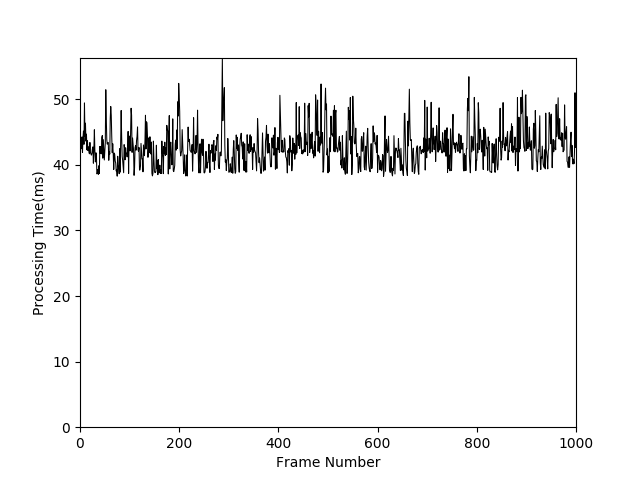
\includegraphics[width=.5\textwidth]{Total_Processing_Time}
  \caption{ Real-time performance of the Raspberry Pi 3 in processing 1000 frames.}
\end{figure}

In our platform, three main real-time tasks are performed during autonomous operation. 
In order, those operations are: (1) capturing and reading the input frame from the designated camera 
or video stream, (2) preprocessing the acquired frame so that it is compatible with the DNN, and (3) 
feeding the frame to, and getting the angle prediction from, the model. However, the time it takes to 
complete each of the operations will differ, with at least one of them being the dominating step in 
processing each frame.

\begin{table}[h]
  \centering
  \begin{tabular} {| l | l | l | l | l |}
    \hline
    \textbf{operation} & \textbf{mean} & \textbf{max} & \textbf{99pct} & \textbf{stdev} \\ \hline 
    Frame Capture & 2.28 & 4.94 & 63.31 &  .51\\ \hline
    Preprocessing & 3.09 & 4.6 & 3.31 & .1 \\ \hline
    Angle Prediction & 37.3 & 51.03 & 45.48 & 2.75 \\ 
    \hline
  \end{tabular}
  \caption{Real-time performance of the Raspberry Pi 3 depending on the number of cores used.}
\end{table}

In order to determine which operation(s) take the longest to execute, we measured the time it 
took for each step to be completed. For this experiment, all four of the Pi's cpu cores were utilized, 
and only one model was run. As is shown in Fig. 1, the angle prediction operation (3) consumes the 
majority of the processing for each frame. Furthermore, the time it takes for the operation to 
complete is volatile, and can range anywhere between 30 ms and 50 ms for any particular frame. On the 
other hand, both the frame capture (1) and preprocessing (2) operations take substantially less time 
and are relatively more consistent in their times, at 2 ms and 3 ms, respectively. 

\subsection{Multicore Performance}
It may not always be the case that all four cores of the Raspberry Pi 3's Cortex A-53 CPU can be used 
solely for the purpose of operating an autonomous vehicle. Thus, we test how the number of cores 
utilized for real-time operations affects the Pi's overall ability to function as an autonomous 
vehicle platform.

\begin{table}[h]
  \centering
  \begin{tabular} {| l | l | l | l | l | l | l | l | l | l |}
    \hline
    \textbf{num cores} & \textbf{mean} & \textbf{max} & \textbf{99pct} & \textbf{stdev} \\ \hline 
    1 & 61.96 & 66 & 63.31 &  .51\\ \hline
    2 & 50.49 & 71.55 & 70.03 & 4.18 \\ \hline
    3 & 48.11 & 72.22 & 58.45 & 2.8 \\ \hline
    4 & 42.67 & 56.37 & 50.70 & 2.8 \\
    \hline
  \end{tabular}
  \caption{Real-time performance of the Raspberry Pi 3 depending on the number of cores used.}
\end{table}

As is depicted in Table 1, the Raspberry Pi performed better, on average, when it utilized more 
cores. With 4 cores, the Pi was able to meet the vast majority of its 50 ms deadlines, doing so in 
almost 99\% of the processed frames. The Pi had the worst average performance when using only 1 core, 
as it was unable to meet any of the 50 ms deadlines (its fastest processing time was just under 60 
ms). Another observation is that the difference between using 2 cores and 3 cores is relatively 
small. On average, using 3 cores only performed better by 2 ms, so the addition of one core in that 
specific case offers relatively little improvement. However, please note that the average time when 
using 3 cores was below the 50 ms deadline, while the average time using 2 cores was slightly above it. 
One important observation that can be made is that of consistency, as using only 1 core had a much 
steadier performance. As a result, the use of multiple cores is very beneficial in terms of reducing 
the time it takes to complete real-time operations, but may ultimately result in processing times 
that are more volatile.

\subsection{Multimodel Performance}
In a real world scenario, it is highly probable that multiple models will need to be used 
simultaneously in order to perform various important tasks (angle prediction, object detection, 
etc.)\cite{}. As such, we also tested the capability of the Raspberry Pi to run multple models at the 
same time, and measure whether all models are able to meet their respective deadlines on a consistent 
basis. Specifically, the Pi is tested in the cases of running 2 and 4 models simultaneously. For each 
case, all models are allocated an equal number of cores, with 2 models having 2 cores each, and 4 
models having 1 core each.

\begin{table*}
  \begin{tabular} {| l | l | l | l | l | l | l | l | l |}
  \hline
  \textbf{num models} & \textbf{cores} & \textbf{mean} & \textbf{L1 refs} & \textbf{L1 
    misses} & \textbf{L1 miss \%} & textbf{L2 refs} & \textbf{L2 misses} & \textbf{L2 miss \%} \\ \hline
  1 & 0,1 & 51.35 & 3.04E+10 & 4.78E+08 & 1.58 & 3.31E+09 & 3.68E+08 & 11.12\\ \hline
  2 & 0,1 & 58.03 & 3.04E+10 & 4.91E+08 & 1.61 & 3.91E+09 & 4.26E+08 & 10.88 \\ \hline
  2 & 2,3 & 56.4 & 3.04E+10 & 4.80E+08 & 1.58 & 3.88E+09 & 4.21E+08 & 10.87 \\ \hline
  \end{tabular}
  \caption{Real-time performance of the Raspberry Pi 3 when 2 models are running simultaneously.}
\end{table*}

Ideally, each model run would replicate a single model run. However, Table 2 shows that such was not 
the case. In the tests where 2 models ran simultaneously, both of the models showed average time 
increases of around 5-7 ms, around 10\%, when compared to a baseline of 1 model running on two cores. 
This change, however, did not seem to be caused by any form of cache interference as both L1 and L2 
cache misses remained constant, regardless of the number of models running. The number of L1 misses 
being close to 1.6\% of all references and the number of L2 misses being about 11\% of all 
references.

\begin{table*}
  \begin{tabular} {| l | l | l | l | l | l | l | l | l |}
  \hline
  \textbf{num models} & \textbf{core} & \textbf{mean} & \textbf{L1 refs} & \textbf{L1 
    misses} & \textbf{L1 miss \%} & textbf{L2 refs} & \textbf{L2 misses} & \textbf{L2 miss \%} \\ \hline
    1 & 0 &  62.48 & 2.78E+10 & 4.36E+08 & 1.57 & 2.83E+09 & 3.59E+08 & 12.68  \\ \hline
    4 & 0 & 77.9 & 2.79E+10 & 4.53E+08 & 1.63 & 3.36E+09 & 4.43E+08 & 13.19 \\ \hline
    4 & 1 & 78.89 & 2.79E+10 & 4.64E+08 & 1.67 & 3.42E+09 & 4.38E+08 & 12.82 \\ \hline
    4 & 2 & 77.81 & 2.78E+10 & 4.45E+08 & 1.6 & 3.45E+09 & 4.41E+08 & 12.77 \\ \hline
    4 & 3 & 77.87 & 2.79E+10 & 4.45E+08 & 1.60 & 3.41E+09 & 4.39E+08 & 12.88 \\ \hline
  \end{tabular}
  \caption{Real-time performance of the Raspberry Pi when 4 models are running simultaneously.}
\end{table*}

The difference was even greater in the case of 4 models running concurrently, as each one displayed 
an average time increase of approximately 15 ms, around 30\%, when compared to a single model 
running on 1 core. Once again, though, cache interference was not a factor as the number of L1 cache 
misses remained 1.6\% of all references, and the number of L2 cache misses stayed at 13\% of all 
references.

\subsection{Performance Requirements}
In the utilization of the Raspberry Pi 3 in our platform, there are a few factors that need to be 
considered and/or enforced in order to guarantee that the Pi is able to consistently perform at a 
desired level. Specifically, these issues all have the potential to negatively affect the cpu clock 
speed/frequency, which would result in decreased performance. While, in the above experiments, the cpu 
operated at a preferred clock speed of 1.2 GHz, it is entirely possible for the cpu to operate at a 
lower frequency if the following problems are not taken into account.

The most notable issue that can affect the cpu clock speed is that of the power supplied to the 
Raspberry Pi. In essence, it is necessary that the Pi be supplied with 2 Amps, as any less could 
hinder the Pi's ability to maintain a 1.2 GHz frequency. In experiments done with a power supply that 
only provided 1 Amp, the Pi was unable to sustain a 1.2 GHz clock speed and, instead, fluctuated 
between operating at 600 MHz and 1.2 GHz. As a result, it is necessary, or at least highly 
recommended, that the power supply used for the Raspberry Pi 3 be capable of outputting 2 Amps, 
otherwise optimal performance isn't guaranteed.

Another factor that can affect clock speed is that of the cpu's temperature. Some model operations can 
be computationally intensive, thus it is possible for the temperature of the cpu to become relatively 
high. This can be especially problematic in situations where multiple models are running 
simultaneously on the Pi. As a consequence, thermal throttling may be used to decrease the clock 
speed so that the cpu temperature stays at a safe level. As such, the Raspberry Pi may not be suited 
for prolonged use, especially in cases where the workload is relatively larger, like running multiple 
models. Rather, the Pi seems to be better suited for running in set periods, after which it is turned 
off or made idle so that the cpu is given time to cool down.
\section{Related Work}
\cite{Bojarski2016}

\section{Conclusion}
%-------------------------------------------------------------------------

\bibliographystyle{plain}
\bibliography{reference}
\end{document}
